\documentclass{article}

\usepackage[utf8]{inputenc}

\usepackage{geometry}
\usepackage{xcolor}
%\usepackage{graphix}
\usepackage{tikz}
\usepackage{mathtools}
\usepackage{pgfplots}
\usepackage{algorithm}
\usepackage[noend]{algpseudocode}
\usepackage{amsmath}
\usepackage{amsfonts}
\usepackage{amssymb}
\usepackage[backend=biber]{biblatex}

\addbibresource{citations.bib}


\renewcommand{\algorithmicrequire}{\textbf{Input:}}
\renewcommand{\algorithmicensure}{\textbf{Output:}}

\definecolor{gradient1}{HTML}{833ab4}
\definecolor{gradient2}{HTML}{fd1d1d}
\definecolor{gradient3}{HTML}{fc8a3b}
\definecolor{gradient4}{HTML}{fcb045}
\definecolor{gradient0}{HTML}{005ab3}


\geometry{top=2cm, bottom=2cm, left=2cm, right=2cm}

\title{Final Project\\ INF236: Parallel Programming\\ Parallel Matrix Multiplication}

\author{Kate\v{r}ina \v{C}\'{i}\v{z}kov\'{a}, Luca Klingenberg}


\begin{document}

\maketitle

\section{Introduction}
Our goal was to implement a matrix multiplication algorithm in parallel.
The standard algorithm has complexity $\mathcal{O}(n^3)$ and is straightforward
to parallelize. We used its implementation as a reference. We compared
it with Strassen's algorithm, which has complexity $\mathcal{O}(n^{\log_2{7}}) \approx \mathcal{O}(n^{2.8073})$,
but requires more memory management.

\section{Files}
\begin{itemize}
    \item \texttt{driver.c} driver allocates matrices, runs the multiplication,
    measures time and verifies results
    \item \texttt{driver.h} includes C libraries
    \item \texttt{cFiles.h} includes \texttt{.c} files with multiplication implementations

    \item \texttt{sequential\_matmul.c} sequential simple matrix multiplication
    \item \texttt{sequential\_strassen.c} sequential Strassen's algorithm
    \item \texttt{parallel\_matmul.c} simple matrix multiplication in parallel
    \item \texttt{parallel\_strassen\_2\_layers.c} two levels of Strassen's algorithm,
    followed by a simple multiplication in parallel
    \item \texttt{parallel\_strassen.c} recursive Strassen's algorithm with parallel
    additions and subtractions
    \item \texttt{z\_order.c} functions for reordering matrix to z-ordering and back
\end{itemize}

\section{Algorithms}
In this section, all the implemented algorithms are explained in further detail. Our implementation is restricted to square matrices as input, but the algorithms could be modified to also work with non-square matrices.

\subsection{Matrix multiplication}
The standard $\mathcal{O}(n^3)$ algorithm is simple: Each element $c_{ij}$ of 
the resulting matrix $\mathbf{C}$ is calculated as $c_{ij} =\sum_k a_{ik} \cdot b_{kj}$.
It is possible to implement the calculation with only three nested for-loops. Matrices are stored row-wise, so it is better to access them in consecutive order, in order to avoid cache misses.
Because of that, we used the implementation shown in algorithm \ref{alg:matmul}. The complexity is still $\mathcal{O}(n^3)$,
but it runs faster in practice than with three nested loops that are indexed in $kij$ order.

\begin{algorithm}[H] 
\caption{matrix multiplication}
\label{alg:matmul}
\begin{algorithmic}[1]
\Require{$\mathbf{A}, \mathbf{B}$} %Input
\Ensure{$\mathbf{C}$ (the resulting matrix)} %Output
\Statex
\Function{matmul}{$\mathbf{A}, \mathbf{B}$}
	\For{$i=0, \ldots, n-1$}
		\For {$j=0, \ldots, n-1$}
			\State {$c[i][j] = 0$}
		\EndFor
		\For{$k=0, \ldots, n-1$}
			\For{$j=0, \ldots, n-1$}
				\State {$c[i][j] += a[i][k] \cdot b[k][j]$}
			\EndFor
		\EndFor
	\EndFor
	\State \Return {$\mathbf{C}$}
\EndFunction
\end{algorithmic}
\end{algorithm}

\subsection{Parallel matrix multiplication}
We just parallelized the outermost loop of the simple matrix multiplication algorithm
described in the previous section with a \texttt{\#pragma omp parallel for} construct.

\subsection{Strassen's algorithm}

The matrix multiplication can be formulated in terms of block matrices:
$$
\mathbf{A} \cdot \mathbf{B} =
\begin{pmatrix}
\mathbf{A}_{00} & \mathbf{A}_{01} \\
\mathbf{A}_{10} & \mathbf{A}_{11} 
\end{pmatrix}
\cdot
\begin{pmatrix}
\mathbf{B}_{00} & \mathbf{B}_{01} \\
\mathbf{B}_{10} & \mathbf{B}_{11} 
\end{pmatrix}
=
\begin{pmatrix}
\mathbf{A}_{00}\mathbf{B}_{00}+\mathbf{A}_{01}\mathbf{B}_{10} & \mathbf{A}_{00}\mathbf{B}_{01}+\mathbf{A}_{01}\mathbf{B}_{11} \\
\mathbf{A}_{10}\mathbf{B}_{00}+\mathbf{A}_{11}\mathbf{B}_{10} & \mathbf{A}_{10}\mathbf{B}_{01}+\mathbf{A}_{11}\mathbf{B}_{11} 
\end{pmatrix}
=
\begin{pmatrix}
\mathbf{C}_{00} & \mathbf{C}_{01} \\
\mathbf{C}_{10} & \mathbf{C}_{11} 
\end{pmatrix}
= \mathbf{C}
$$

According to this formula, it needs 8 multiplications of half-sized matrices. 
The idea of Strassen's algorithm is to use more additions and subtractions,
but only 7 multiplications of half-sized matrices. Then, the algorithm is used recursively
for these multiplications. You can see a pseudocode of Strassen's algorithm below.

\begin{algorithm}[H] 
\caption{Strassen's matrix multiplication}
\label{alg:strassen}
\begin{algorithmic}[1]
\Require{$\mathbf{A}, \mathbf{B}$} %Input
\Ensure{$\mathbf{C}$ (the resulting matrix)} %Output
\Statex
\Function{strassen}{$\mathbf{A}, \mathbf{B}, n$}
	\If {n == cutoff}
		\State \Return \Call{matmul}{$\mathbf{A}, \mathbf{B}$}
	\EndIf
	\State {$\mathbf{P}_1 = \Call{strassen}{\mathbf{A}_{00} + \mathbf{A}_{11},  \mathbf{B}_{00} + \mathbf{B}_{11}, \frac{n}{2}$}}
	\State {$\mathbf{P}_2 = \Call{strassen}{\mathbf{A}_{10} + \mathbf{A}_{11},  \mathbf{B}_{00}, \frac{n}{2}$}}
	\State {$\mathbf{P}_3 = \Call{strassen}{\mathbf{A}_{00},  \mathbf{B}_{01} - \mathbf{B}_{11}, \frac{n}{2}$}}
	\State {$\mathbf{P}_4 = \Call{strassen}{\mathbf{A}_{11},  \mathbf{B}_{10} - \mathbf{B}_{00}, \frac{n}{2}$}}
	\State {$\mathbf{P}_5 = \Call{strassen}{\mathbf{A}_{00} + \mathbf{A}_{01},  \mathbf{B}_{11}, \frac{n}{2}$}}
	\State {$\mathbf{P}_6 = \Call{strassen}{\mathbf{A}_{10} - \mathbf{A}_{00},  \mathbf{B}_{00} + \mathbf{B}_{01}, \frac{n}{2}$}}
	\State {$\mathbf{P}_7 = \Call{strassen}{\mathbf{A}_{01} - \mathbf{A}_{11},  \mathbf{B}_{10} + \mathbf{B}_{11}, \frac{n}{2}$}}
	\State {$\mathbf{C}_{00} = \mathbf{P}_1 + \mathbf{P}_4 - \mathbf{P}_5 + \mathbf{P}_7$}
	\State {$\mathbf{C}_{01} = \mathbf{P}_3 + \mathbf{P}_5$}
	\State {$\mathbf{C}_{10} = \mathbf{P}_2 + \mathbf{P}_4$}
	\State {$\mathbf{C}_{11} = \mathbf{P}_1 - \mathbf{P}_2 + \mathbf{P}_3 + \mathbf{P}_6$}
	 	
	\State \Return {$\mathbf{C}$}
\EndFunction
\end{algorithmic}
\end{algorithm}

There are 18 additions and subtractions calculated in Strassen's algorithm. 
We used Winograd's version of Strassen's algorithm described in \cite{boyer2009memory}.
It needs only 15 additions and subtractions because some results are reused.
We also used scheduling table 1 from the same paper. 
Therefore our implementation needs only two temporary matrices in each recursive call to store intermediate results.
Strassen's algorithm is recursive and it is working with quarters of input matrices. 
Because of that, it is useful to use some recursive ordering for storing matrices in memory, for example z-ordering (figures \ref{z_diagram}, \ref{z_mem}).
If the dimension of the input matrices is not a power of two, the input matrices are zero-padded to a size of the next larger power of two.

\begin{figure}[htbp]
\centerline{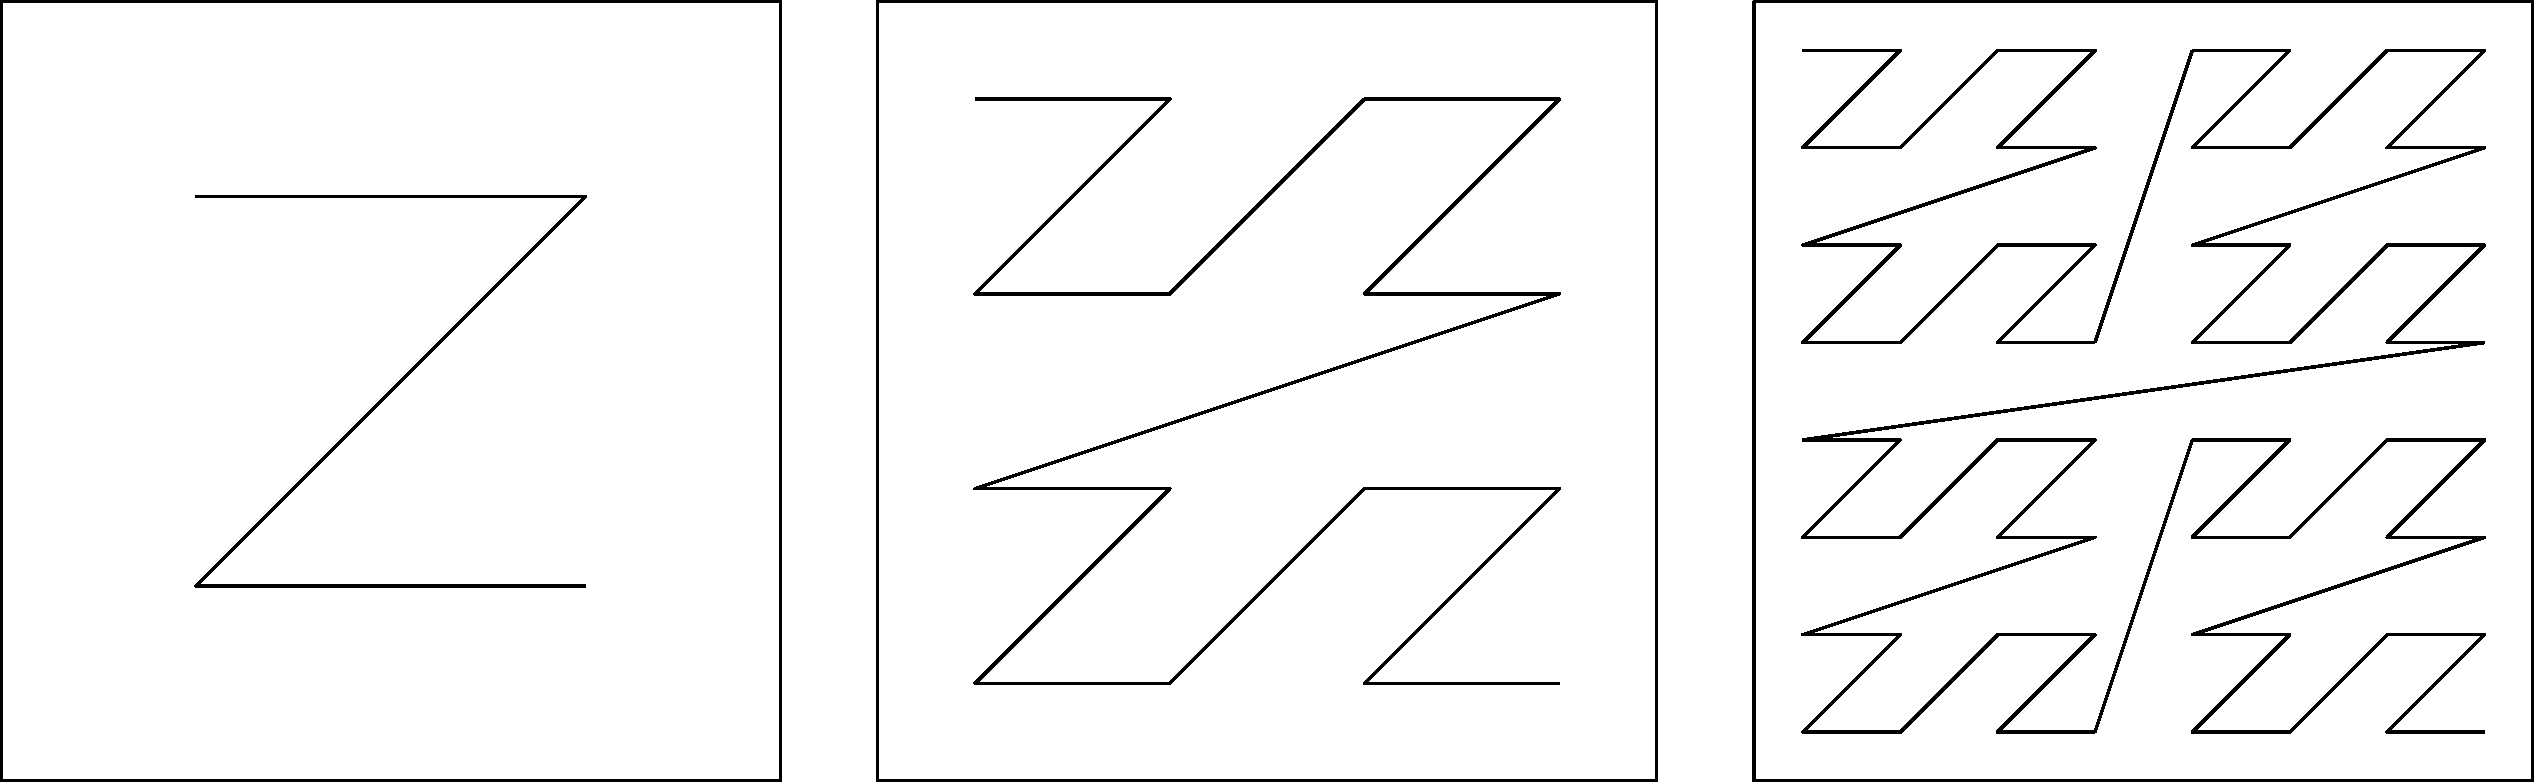
\includegraphics[scale=.3]{z_ordering.pdf}}
\caption{z-ordering diagram}
\label{z_diagram}
\end{figure}

\begin{figure}[htbp]
\centerline{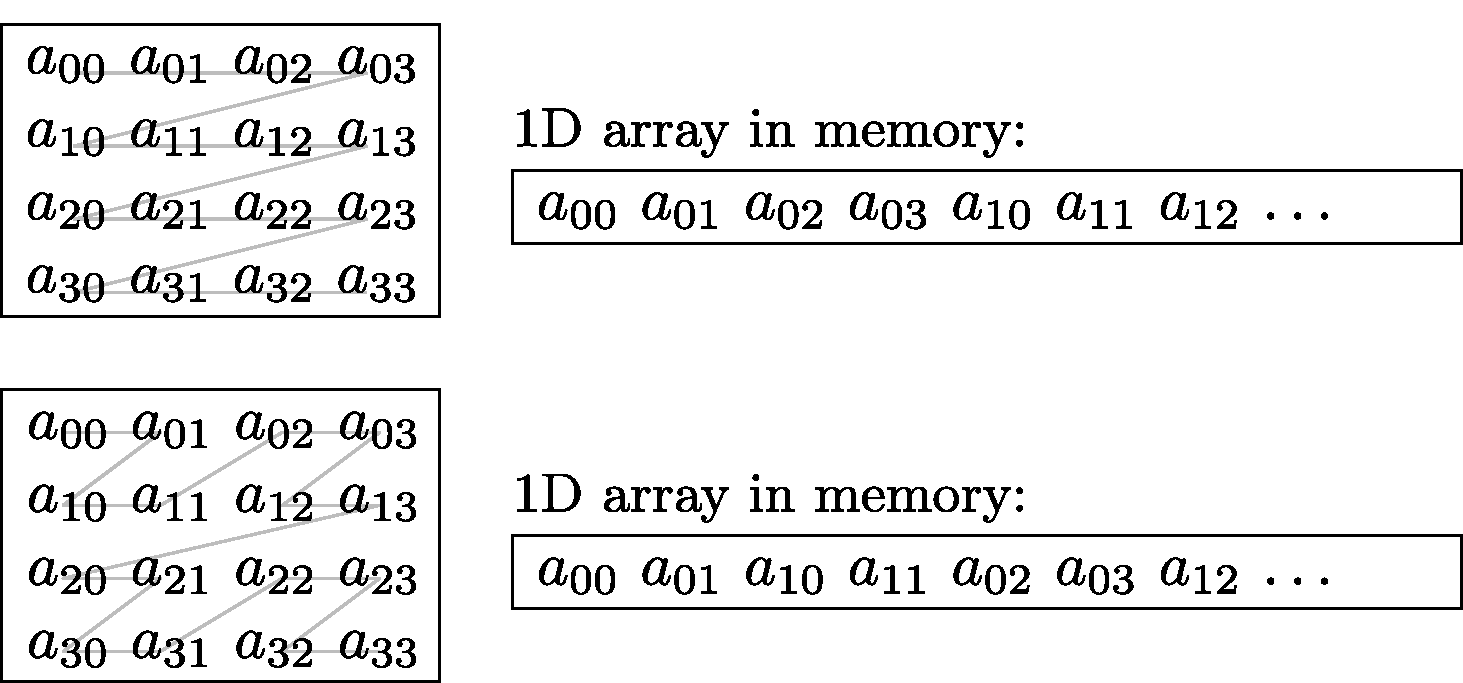
\includegraphics[scale=.35]{mem_ordering.pdf}}
\caption{row-ordered and z-ordered matrix stored in memory}
\label{z_mem}
\end{figure}

Its advantage is, that all submatrices are stored in consecutive parts of the memory.
However, we switch from Strassen's algorithm to the simple matrix multiplication algorithm,
since the overhead of Strassen's algorithm is getting too big for smaller matrix sizes.
For the simple matrix multiplication it is better to have the matrices ordered row-wise.
In our implementation, we combined both z-ordering and usual row-by-row ordering.
We used the z-ordering for bigger submatrices, but
we left the small submatrices which are multiplied with the simple multiplication algorithm
in row-wise order (figure \ref{z_partly}). The functions for reordering matrices to this layout
and back are implemented in \texttt{z\_order.c} file.

\begin{figure}[htbp]
\centerline{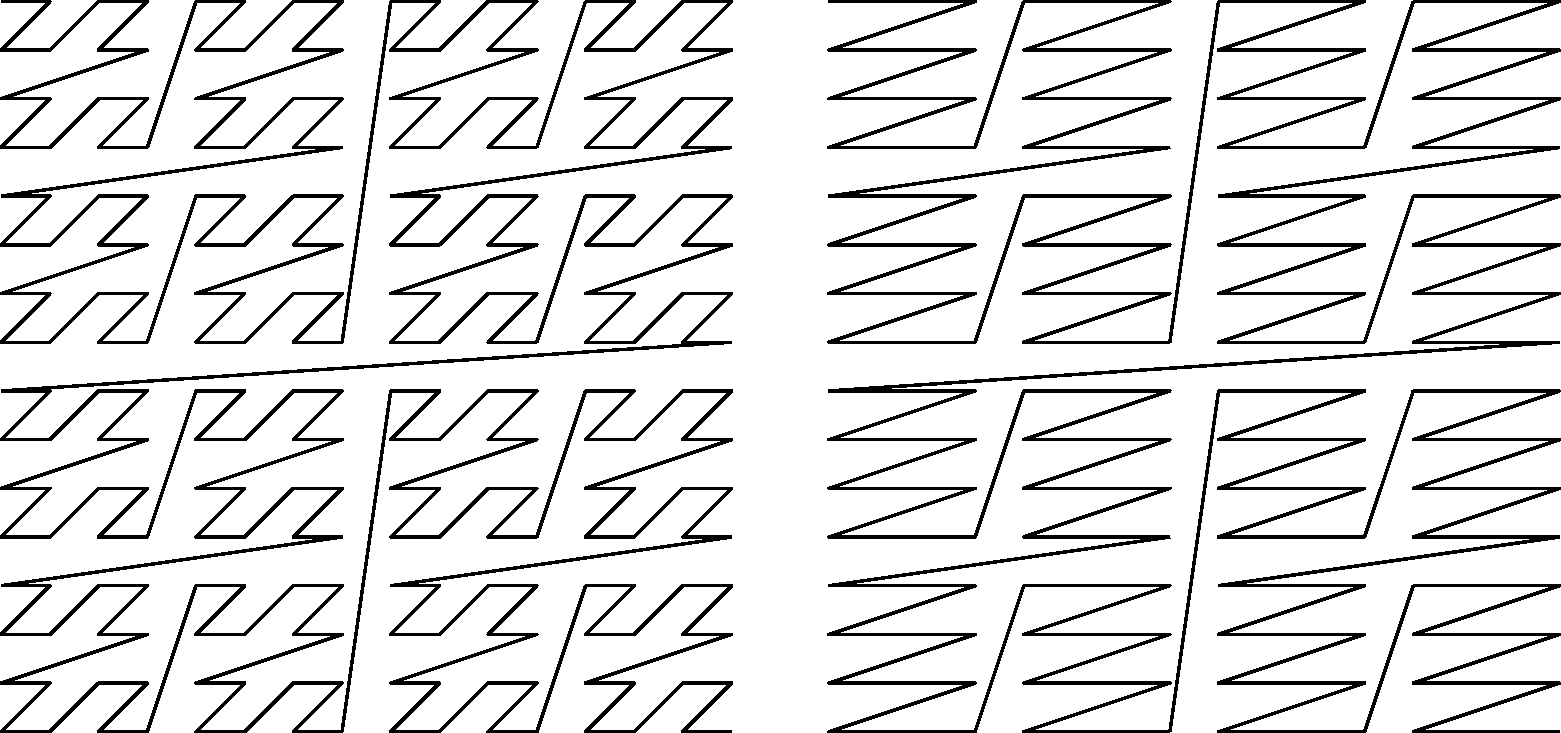
\includegraphics[scale=.5]{partly_z_ordering.pdf}}
\caption{z-ordering only for bigger submatrices}
\label{z_partly}
\end{figure}


\subsection{Parallel Strassen's algorithm}

It is straightforward to parallelize additions and subtractions in Strassen's algorithm.
The problem is, that for small matrices it is not worth it to initialize a parallel region.
Because of that, we can not just insert a \texttt{\#pragma omp parallel for} construct before
the addition and subtraction for-loop.

Then, we were thinking about parallelizing recursive calls -- calculate $\mathbf{P}_1, \ldots, \mathbf{P}_7$ in parallel.
But since we are using only two temporary matrices in each recursive call, it is necessary to finish
a recursive call before starting the next one. This may be solved using more space for intermediate
results, but we did not try that.

We decided to try some number of recursive steps and then switch to the parallelized simple matrix multiplication.

\subsubsection{2-layers parallel Strassen's algorithm}

This implementation uses two levels of Strassen's algorithm (hardcoded as functions 
\texttt{parallel\_strassen\_level\_1} and \texttt{parallel\_strassen\_level\_2}). There are seven
parallel regions initialized for additions and subtractions in level 1 and only one for 
all additions, subtractions and multiplications in level 2.

\subsubsection{Recursive parallel Strassen's algorithm with matrix size cutoff}
After some measurements with 2-layers parallel Strassen's algorithm, we implemented this variant.
The idea is the same, but there are more recursive calls of Strassen's algorithm with parallelized
additions and subtractions (similar to \texttt{parallel\_strassen\_level\_1}). 
When the cutoff matrix size is reached, we switch to the parallelized simple matrix multiplication. We tried several cutoff sizes
and a cutoff size of 512$\times$512 was the most promising one.

Since there are at least two layers of Strassen's algorithm and we set the cutoff to 512$\times$512,
we need to solve cases when the matrices are smaller than 2048$\times$2048. In these cases, we only use the 
parallelized simple matrix multiplication.

\section{Experiments}

We ran all the experiments on the machine available at \texttt{brake.ii.uib.no}.

\subsection{Sequential Strassen's algorithm}

Strassen's algorithm theoretically runs recursively until submatrices reach dimension 1, such that the matrix multiplication just becomes a multiplication of two scalars.
However, it is in practice faster to stop the recursion at a higher level, because for smaller matrix sizes, Strassen's algorithm performs worse than the standard matrix multiplication algorithm. Therefore, we experimented with different cutoff levels for different matrix sizes. The results can be seen in figure \ref{fig:cutoff_levels}. We found that the algorithm performs best when the submatrix size at the cutoff has dimension $64 \times 64$.

	
% Comparing different cutoff levels of sequential Strassen
\begin{figure}[h!]
\center
\begin{tikzpicture}
\begin{axis}[
    xlabel={submatrix dimension at cuttoff},
    ylabel={speedup},
    xmin=0, xmax=512,
    ymin=0, ymax=4,
    xtick={1, 2, 4, 8, 16, 32, 64, 128, 256, 512},
    xticklabels={1, 2, 4, 8, 16, 32, 64, 128, 256},
    ytick={0, 0.5, 1, 1.5, 2, 2.5, 3, 3.5, 4},
	xmode=log,
    log basis x={2},
    legend pos=outer north east,
    xmajorgrids=true,
    ymajorgrids=true,
    grid style=dashed,
]

	% running time of normal sequential: 22.729855
	\addplot[color=gradient1, mark=*, only marks] table [x=cutoff, y=size1, col sep=comma] {cutoffs.csv};
	% running time of normal sequential: 1.397876
	\addplot[color=gradient2, mark=*, only marks] table [x=cutoff, y=size2, col sep=comma] {cutoffs.csv};
	% running time of normal sequential: 0.177942
	\addplot[color=gradient3, mark=*, only marks] table [x=cutoff, y=size3, col sep=comma] {cutoffs.csv};
	% running time of normal sequential: 0.032513
	\addplot[color=gradient4, mark=*, only marks] table [x=cutoff, y=size4, col sep=comma] {cutoffs.csv};

    \legend{2048 $\times$ 2048, 1024 $\times$ 1024, 512 $\times$ 512, 256 $\times$ 256}
\end{axis}
\end{tikzpicture}
\caption{Sequential Strassen's algorithm with different values for the cutoff level}
\label{fig:cutoff_levels}
\end{figure}

\subsection{Comparison of parallel matrix multiplication and parallel Strassen's algorithm to the
sequential Strassen's algorithm with different amount of threads}

Next, we compared all parallel algorithms using different amount of threads. The submatrix dimension at the cutoff level was 32 $\times$ 32, which is not optimal 



% Compare different number of threads for 256x256
\begin{figure}[h!]
\center
\begin{tikzpicture}
\begin{axis}[
    xlabel={\#threads},
    ylabel={speedup},
    xmin=0, xmax=8,
    ymin=0, ymax=26,
    xtick={0, 1, 2, 3, 4, 5, 6, 7},
    xticklabels={0, 1, 2, 5, 10, 20, 40, 60},
    ytick={0, 5, 10, 15, 20, 25},
    legend pos=outer north east,
    xmajorgrids=true,
    ymajorgrids=true,
    grid style=dashed,
]
	
	\addplot[color=gradient1, mark=*, only marks] table [x=config, y=strassen_vs_simple_parallel, col sep=comma] {result256.csv};
	
	\addplot[color=gradient2, mark=*, only marks] table [x=config, y=strassen_vs_strassen_2layers, col sep=comma] {result256.csv};
	
	\addplot[color=gradient4, mark=*, only marks] table [x=config, y=strassen_vs_strassen_recursive, col sep=comma] {result256.csv};
    
    \legend{parallel matmul, parallel 2 layers Strassen, parallel recursive Strassen}

\end{axis}
\end{tikzpicture}
\caption{Comparing different variants of Strassen's algorithm with matrix size 256 $\times$ 256}
\label{fig:strassen_cmp_256}
\end{figure}

% Compare different number of threads for 512x512
\begin{figure}[h!]
\center
\begin{tikzpicture}
\begin{axis}[
    title={Matrices size 512 $\times$ 512},
    xlabel={\#threads},
    ylabel={speedup},
    xmin=0, xmax=8,
    ymin=0, ymax=18,
    xtick={0, 1, 2, 3, 4, 5, 6, 7},
    xticklabels={0, 1, 2, 5, 10, 20, 40, 60},
    ytick={0, 5, 10, 15},
    legend pos=outer north east,
    xmajorgrids=true,
    ymajorgrids=true,
    grid style=dashed,
]

	
	\addplot[color=gradient1, mark=*, only marks] table [x=config, y=strassen_vs_simple_parallel, col sep=comma] {result512.csv};
	
	\addplot[color=gradient2, mark=*, only marks] table [x=config, y=strassen_vs_strassen_2layers, col sep=comma] {result512.csv};
	
	\addplot[color=gradient4, mark=*, only marks] table [x=config, y=strassen_vs_strassen_recursive, col sep=comma] {result512.csv};

	\legend{parallel matmul, parallel 2 layers Strassen, parallel recursive Strassen}

\end{axis}
\end{tikzpicture}
\caption{Comparing different variants of Strassen's algorithm with matrix size 512 $\times$ 512}
\label{fig:strassen_cmp_512}
\end{figure}

% Compare different number of threads for 1024x1024
\begin{figure}[h!]
\center
\begin{tikzpicture}
\begin{axis}[
    title={Matrices size 1024 $\times$ 1024},
    xlabel={\#threads},
    ylabel={speedup},
    xmin=0, xmax=8,
    ymin=0, ymax=18,
    xtick={0, 1, 2, 3, 4, 5, 6, 7},
    xticklabels={0, 1, 2, 5, 10, 20, 40, 60},
    ytick={0, 5, 10, 15},
    legend pos=outer north east,
    xmajorgrids=true,
    ymajorgrids=true,
    grid style=dashed,
]

	
	\addplot[color=gradient1, mark=*, only marks] table [x=config, y=strassen_vs_simple_parallel, col sep=comma] {result1024.csv};
	
	\addplot[color=gradient2, mark=*, only marks] table [x=config, y=strassen_vs_strassen_2layers, col sep=comma] {result1024.csv};
	
	\addplot[color=gradient4, mark=*, only marks] table [x=config, y=strassen_vs_strassen_recursive, col sep=comma] {result1024.csv};
    
    \legend{parallel matmul, parallel 2 layers Strassen, parallel recursive Strassen}
\end{axis}
\end{tikzpicture}
\caption{Comparing different variants of Strassen's algorithm with matrix size 1024 $\times$ 1024}
\label{fig:strassen_cmp_1024}
\end{figure}

% Compare different number of threads for 2048x2048
\begin{figure}[h!]
\center
\begin{tikzpicture}
\begin{axis}[
    title={Matrices size 2048 $\times$ 2048},
    xlabel={\#threads},
    ylabel={speedup},
    xmin=0, xmax=8,
    ymin=0, ymax=18,
    xtick={0, 1, 2, 3, 4, 5, 6, 7},
    xticklabels={0, 1, 2, 5, 10, 20, 40, 60},
    ytick={0, 5, 10, 15},
    legend pos=outer north east,
    xmajorgrids=true,
    ymajorgrids=true,
    grid style=dashed,
]

	
	\addplot[color=gradient1, mark=*, only marks] table [x=config, y=strassen_vs_simple_parallel, col sep=comma] {result2048.csv};
	
	\addplot[color=gradient2, mark=*, only marks] table [x=config, y=strassen_vs_strassen_2layers, col sep=comma] {result2048.csv};
	
	\addplot[color=gradient4, mark=*, only marks] table [x=config, y=strassen_vs_strassen_recursive, col sep=comma] {result2048.csv};

    \legend{parallel matmul, parallel 2 layers Strassen, parallel recursive Strassen}

\end{axis}
\end{tikzpicture}
\caption{Comparing different variants of Strassen's algorithm with matrix size 2048 $\times$ 2048}
\label{fig:strassen_cmp_2048}
\end{figure}

% Compare different number of threads for 4096x4096
\begin{figure}[h!]
\center
\begin{tikzpicture}
\begin{axis}[
    title={Matrices size 4096 $\times$ 4096},
    xlabel={\#threads},
    ylabel={speedup},
    xmin=0, xmax=8,
    ymin=0, ymax=18,
    xtick={0, 1, 2, 3, 4, 5, 6, 7},
    xticklabels={0, 1, 2, 5, 10, 20, 40, 60},
    ytick={0, 5, 10, 15},
    legend pos=outer north east,
    xmajorgrids=true,
    ymajorgrids=true,
    grid style=dashed,
]

	
	\addplot[color=gradient1, mark=*, only marks] table [x=config, y=strassen_vs_simple_parallel, col sep=comma] {result4096.csv};
	
	\addplot[color=gradient2, mark=*, only marks] table [x=config, y=strassen_vs_strassen_2layers, col sep=comma] {result4096.csv};
	
	\addplot[color=gradient4, mark=*, only marks] table [x=config, y=strassen_vs_strassen_recursive, col sep=comma] {result4096.csv};

    \legend{parallel matmul, parallel 2 layers Strassen, parallel recursive Strassen}

\end{axis}
\end{tikzpicture}
\caption{Comparing different variants of Strassen's algorithm with matrix size 4096 $\times$ 4096}
\label{fig:strassen_cmp_4096}
\end{figure}

% Compare different number of threads for 8192x8192
\begin{figure}[h!]
\center
\begin{tikzpicture}
\begin{axis}[
    title={Matrices size 8192 $\times$ 8192},
    xlabel={\#threads},
    ylabel={speedup},
    xmin=0, xmax=8,
    ymin=0, ymax=18,
    xtick={0, 1, 2, 3, 4, 5, 6, 7},
    xticklabels={0, 1, 2, 5, 10, 20, 40, 60},
    ytick={0, 5, 10, 15},
    legend pos=outer north east,
    xmajorgrids=true,
    ymajorgrids=true,
    grid style=dashed,
]

	
	\addplot[color=gradient1, mark=*, only marks] table [x=config, y=strassen_vs_simple_parallel, col sep=comma] {result8192.csv};
	
	\addplot[color=gradient2, mark=*, only marks] table [x=config, y=strassen_vs_strassen_2layers, col sep=comma] {result8192.csv};
	
	\addplot[color=gradient4, mark=*, only marks] table [x=config, y=strassen_vs_strassen_recursive, col sep=comma] {result8192.csv};
	
	\legend{parallel matmul, parallel 2 layers Strassen, parallel recursive Strassen}
    
\end{axis}
\end{tikzpicture}
\caption{Comparing different variants of Strassen's algorithm with matrix size 8192 $\times$ 8192}
\label{fig:strassen_cmp_8192}
\end{figure}

\subsection{Running times for all implemented algorithms and different numbers of threads}

% Running time for 8192
\begin{figure}[h!]
\center
\begin{tikzpicture}
\begin{semilogyaxis}[
    title={Matrices size 8192 $\times$ 8192},
    xlabel={\#threads},
    ylabel={running time in seconds},
    xmin=0, xmax=8,
    ymin=0, ymax=2500,
    xtick={0, 1, 2, 3, 4, 5, 6, 7},
    xticklabels={0, 1, 2, 5, 10, 20, 40, 60},
    legend pos=outer north east,
    xmajorgrids=true,
    ymajorgrids=true,
    grid style=dashed,
]

    \addplot[color=gradient0, mark=*] table [x=config, y=simple, col sep=comma] {result8192.csv};
	
	\addplot[color=gradient1, mark=*] table [x=config, y=strassen, col sep=comma] {result8192.csv};
	
	\addplot[color=gradient2, mark=*, only marks] table [x=config, y=simple_parallel, col sep=comma] {result8192.csv};
	
	\addplot[color=gradient3, mark=*, only marks] table [x=config, y=strassen_2layers, col sep=comma] {result8192.csv};
	
	\addplot[color=gradient4, mark=*, only marks] table [x=config, y=strassen_recursive, col sep=comma] {result8192.csv};
    
    \legend{matmul, Strassen, parallel matmul, parallel 2 layers Strassen, parallel recursive Strassen }

\end{semilogyaxis}
\end{tikzpicture}

\end{figure}

\subsection{All implemented algorithms for different sizes of matrices}

\begin{figure}[h!]
\center
\begin{tikzpicture}
\begin{semilogyaxis}[
    title={Running time with 40 threads},
    xlabel={matrix size},
    ylabel={running time in seconds},
    ymin=0, ymax=400,
    legend pos=outer north east,
    xmajorgrids=true,
    ymajorgrids=true,
    grid style=dashed,
]

    \addplot[color=gradient0, mark=*, only marks] table [x=size, y=simple, col sep=comma] {results_diff_size.csv};
	
	\addplot[color=gradient1, mark=*, only marks] table [x=size, y=strassen, col sep=comma] {results_diff_size.csv};
	
	\addplot[color=gradient2, mark=*, only marks] table [x=size, y=simple_parallel, col sep=comma] {results_diff_size.csv};
	
	\addplot[color=gradient3, mark=*, only marks] table [x=size, y=strassen_2layers, col sep=comma] {results_diff_size.csv};
	
	\addplot[color=gradient4, mark=*, only marks] table [x=size, y=strassen_recursive, col sep=comma] {results_diff_size.csv};
    
    \legend{matmul, strassen, parallel matmul, parallel 2 layers strassen, parallel recursive strassen }
\end{semilogyaxis}
\end{tikzpicture}

\end{figure}

\begin{figure}[h!]
\center
\begin{tikzpicture}
\begin{axis}[
    title={Speedup with respect to simple matrix multiplication},
    xlabel={matrix size},
    ylabel={running time in seconds},
    ymin=0, ymax=65,
    legend pos=outer north east,
    xmajorgrids=true,
    ymajorgrids=true,
    grid style=dashed,
]
	
	\addplot[color=gradient0, mark=*, only marks] table [x=size, y=speedup_strassen, col sep=comma] {results_diff_size.csv};
	
	\addplot[color=gradient1, mark=*, only marks] table [x=size, y=speedup_simple_parallel, col sep=comma] {results_diff_size.csv};
	
	\addplot[color=gradient2, mark=*, only marks] table [x=size, y=speedup_strassen_2layers, col sep=comma] {results_diff_size.csv};
	
	\addplot[color=gradient4, mark=*, only marks] table [x=size, y=speedup_strassen_recursive, col sep=comma] {results_diff_size.csv};
    
    \legend{strassen, parallel matmul, parallel 2 layers strassen, parallel recursive strassen }
\end{axis}
\end{tikzpicture}

\end{figure}

\section{Conclusion}

\printbibliography

\end{document}